\documentclass[11pt]{aghdpl}
% \documentclass[en,11pt]{aghdpl}  % praca w języku angielskim

% Lista wszystkich języków stanowiących języki pozycji bibliograficznych użytych w pracy.
% (Zgodnie z zasadami tworzenia bibliografii każda pozycja powinna zostać utworzona zgodnie z zasadami języka, w którym dana publikacja została napisana.)
\usepackage[english,polish]{babel}

% Użyj polskiego łamania wyrazów (zamiast domyślnego angielskiego).
\usepackage{polski}

\usepackage[utf8]{inputenc}

% dodatkowe pakiety
\usepackage{graphicx}
\DeclareGraphicsExtensions{.png, .jpg}
\graphicspath{ {./img/} }

\usepackage{mathtools}
\usepackage{amsfonts}
\usepackage{amsmath}
\usepackage{amsthm}
\usepackage{longtable}

\usepackage{listings}
\usepackage{color}

\definecolor{purple}{rgb}{0.7,0.1,0.40}

\lstset{
	frame=tb,
	aboveskip=3mm,
	belowskip=3mm,	
	language=Matlab,%
    %basicstyle=\color{red},
    breaklines=true,%
    morekeywords={matlab2tikz},
    keywordstyle=\color{blue},%
    morekeywords=[2]{1}, keywordstyle=[2]{\color{black}},
    identifierstyle=\color{black},%
    stringstyle=\color{purple},
    commentstyle=\color{green},%
    showstringspaces=false,%without this there will be a symbol in the places where there is a space
    numbers=left,%
    numberstyle={\tiny \color{black}},% size of the numbers
    numbersep=9pt % this defines how far the numbers are from the text
}

% ------------------------
% --- < listingi > ---

% Użyj czcionki kroju Courier.
\usepackage{courier}

\usepackage{listings}
\lstloadlanguages{TeX}

\lstset{
	literate={ą}{{\k{a}}}1
           {ć}{{\'c}}1
           {ę}{{\k{e}}}1
           {ó}{{\'o}}1
           {ń}{{\'n}}1
           {ł}{{\l{}}}1
           {ś}{{\'s}}1
           {ź}{{\'z}}1
           {ż}{{\.z}}1
           {Ą}{{\k{A}}}1
           {Ć}{{\'C}}1
           {Ę}{{\k{E}}}1
           {Ó}{{\'O}}1
           {Ń}{{\'N}}1
           {Ł}{{\L{}}}1
           {Ś}{{\'S}}1
           {Ź}{{\'Z}}1
           {Ż}{{\.Z}}1,
	basicstyle=\footnotesize\ttfamily,
}

% ------------------------

\AtBeginDocument{
	\renewcommand{\tablename}{Tabela}
	\renewcommand{\figurename}{Rys.}
}

% ------------------------
% --- < tabele > ---

\usepackage{array}
\usepackage{tabularx}
\usepackage{multirow}
\usepackage{booktabs}
\usepackage{makecell}
\usepackage[flushleft]{threeparttable}
\usepackage{siunitx}

% defines the X column to use m (\parbox[c]) instead of p (`parbox[t]`)
\newcolumntype{C}[1]{>{\hsize=#1\hsize\centering\arraybackslash}X}


%---------------------------------------------------------------------------

\author{Filip Pasternak}
\shortauthor{F. Pasternak}

\titlePL{Akwizycja danych dla identyfikacji prostego modelu opad-odpływ.}
\titleEN{Data acquisition for identification of a simple rainfall runoff model.}
\title{Praca inżynierska}

\shorttitlePL{Akwizycja danych dla identyfikacji prostego modelu opad-odpływ.} % skrócona wersja tytułu jeśli jest bardzo długi
\shorttitleEN{Data acquisition for identification of a simple rainfall runoff model.}

\thesistype{Praca dyplomowa inżynierska}

\supervisor{dr inż. Janusz Miller}
%\supervisor{Janusz Miller PhD}

\degreeprogramme{Informatyka}
%\degreeprogramme{Computer Science}

\date{2016}

\department{Katedra Informatyki Stosowanej}
%\department{Department of Applied Computer Science}

\faculty{Wydział Elektrotechniki, Automatyki,\protect\\[-1mm] Informatyki i Inżynierii Biomedycznej}
%\faculty{Faculty of Electrical Engineering, Automatics, Computer Science and Biomedical Engineering}

\acknowledgements{Work hard and never give up! \\ 
Bardzo dziękuję mojemu promotorowi za okazaną pomoc przy tworzeniu tej pracy.}


\setlength{\cftsecnumwidth}{10mm}

%---------------------------------------------------------------------------
\setcounter{secnumdepth}{4}

\begin{document}

\titlepages

% Ponowne zdefiniowanie stylu `plain`, aby usunąć numer strony z pierwszej strony spisu treści i poszczególnych rozdziałów.
\fancypagestyle{plain}
{
	% Usuń nagłówek i stopkę
	\fancyhf{}
	% Usuń linie.
	\renewcommand{\headrulewidth}{0pt}
	\renewcommand{\footrulewidth}{0pt}
}

\tableofcontents
\clearpage

\newpage
\chapter{Wstęp}
\section{Przedmowa}
Natura to nieposkromiona siła, którą człowiek stara się poznać. Choć już od lat 60-tych prowadzone są badania nad systemami modyfikacji pogody (w szczególności do zastosowań militarnych), to prawidłowe przewidywanie zjawisk atmosferycznych, a także ich skutków, wciąż stanowi problem wymagający rozwiązania.

W lecie 2010 roku Polskę zaatakowała ogromna powódź, która dotknęła niemal wszystkich województw. W wyniku wzmożonych opadów rzeki wezbrały i w wielu miejscach wystąpiły z koryta. Mimo istnienia około stu zbiorników retencyjnych oraz wielu zapór wodnych, nie udało się zapobiec tragedii, w~wyniku której mnóstwo ludzi straciło swój dobytek.

Istniejąca obecnie infrastruktura dokonująca pomiarów zjawisk pogodowych czy stanów zbiorników wodnych może stanowić bazę do systemów umożliwiających zapobieganie takim tragediom. Analiza wielkości opadu oraz przewidywanie drogi jej spływu może pozwolić na przykład operatorom zapór wodnych na podjęcie właściwych, a~przede wszystkim odpowiednio wczesnych działań tak, aby przygotować zbiorniki retencyjne na przyjęcie dodatkowej ilości wody oraz w~sposób kontrolowany pokierować jej spływ i zabezpieczyć ludność.

Praca ta traktować będzie o~elemencie składowym przybliżonego powyżej rozwiązania, czyli analizie danych opadowych.

\section{Opis dokumentu}
% Sekcja do rozbudowy w miarę rozszerzenia dokumentu.
Praca ta porusza tematykę analizy danych opadowych pochodzących z~posterunków opadowych. Opisuje teorię przekształcenia wartości punktowej opadu na wartość powierzchniową w~obszarze wskazanej zlewni rzeki.

\textbf{Odczyt danych} rozdział ten opisuje proces przeprowadzonej analizy serwisu w~celu dostępu do danych meteorologicznych i hydrologicznych.

\textbf{Interpolacja danych punktowych opadów} w tej części opisano algorytm triangulacji metodą Delaunaya oraz sposób przekształcenia wartości punktowych opadów na obszar zlewni.
\section{Cele pracy}
\label{sec:cele}
Celem pracy jest analiza możliwości uzyskania danych pogodowych, zbudowanie mechanizmu przekształcającego wskazania z~posterunków opadowych na objętość opadu w~zadanym obszarze, a~także przeprowadzenie badania wpływu usunięcia poszczególnych posterunków na wartości wynikowe.

%Celem pracy jest analiza korelacji danych opadowych i~odpływowych na rzece. Obliczenia opierać się będą na informacjach ze strony pogodynka.pl udostępnianej przez Instytut Meteorologii i Gospodarki Wodnej. Wszelkie działania i obliczenia przeprowadzone zostaną w~środowisku Matlab (darmowa wersja próbna R2015b). Elementy składowe pracy to:
\begin{itemize}
\item
Odczyt z serwisu pogodynka.pl danych posterunków opadowych i wodowskazowych (takich jak nazwa i lokalizacja), wartości odpowiednich wskazań posterunków oraz parametrów granic zlewni.
\item
Przekształcenie danych opadowych metodą triangulacji Delaunaya i aplikacja tej metody do przebiegu granic zlewni.
\item
Analiza korelacji opadu powierzchniowego z~wysokością poziomu wody na odpowiednich posterunkach wodowskazowych.
\end{itemize}
\chapter{Odczyt danych pogodowych}
Posterunki opadowe i~innego rodzaju podobna infrastruktura jest własnością Instytutu Meteorologii i Gospodarki Wodnej. Oferuje on serwis internetowy prezentujący liczne dane meteorologiczne oraz hydrologiczne.

W ramach pracy nad niniejszym projektem, wspomniany wyżej serwis został poddany analizie celem automatycznego odczytu danych, które dalej mogłyby być poddane przetworzeniu. Zostały przygotowane narzędzia odczytujące dane o~posterunkach opadowych i~wodowskazowych (jak nazwa, lokalizacja) oraz ich wartości pomiarowe, a~także informacje o~przebiegu granic poszczególnych zlewni rzek.

W przypadku posterunków opadowych zapisywano wartości ostatniego pomiaru godzinowego i dobowego, a także kolekcje pomiarów godzinowych za ostatnie 48 godzin oraz dobowych za okres tygodnia. Wszystkie w~jednostce mm.

Dane pojedynczego posterunku wodowskazowego składały się z aktualnego wskazania poziomu wody (wraz z datą pomiaru), kolekcji godzinowych pomiarów poziomu wody za ostatnie 72 godziny(w jednostce cm) i~godzinowych pomiarów wielkości przepływu (w jednostce $m^3/s$) za taki sam okres czasu.


Z powodu obostrzeń prawnych zawartych w~\textbf{Zasadach użytkowania serwisu internetowego IMGW PIB} nie można jednak wykorzystać rzeczywistych danych pobieranych z~serwisu na potrzeby pracy. Zgodnie z~\textsection~2~ust.~5 warunkiem koniecznym jest uzyskanie pisemnej zgody Instytutu. Złożone zostało odpowiednie podanie, a~także przeprowadzono spotkanie z~Zastępcą Kierownika Centrum Hydrologicznej Osłony Kraju, Radosławem Doktorem. Podczas rozmowy dowiedziano się, iż warunkiem koniecznym uzyskania dostępu do danych IMGW, na potrzeby pracy podobnej jak niniejsza, jest zawarcie umowy między Instytutem a Uczelnią. Kolejnym punktem są pozwolenia w~kontekście konkretnego projektu, gdzie należy precyzyjnie określić między innymi rodzaj oczekiwanych danych oraz obszar jakiego mają dotyczyć. Po pozytywnym rozpatrzeniu prośby rozpoczęte zostają prace nad indywidualnym API przekazującym wskazane informacje. Reasumując, okres oczekiwania na wyrażenie zgody i~dalej stworzenie odpowiedniego interfejsu to co najmniej kilka miesięcy.

Ponieważ nie uzyskano zgody na użycie w~pracy danych rzeczywistych przeprowadzenie analizy korelacji wyznaczanych wartości opadu powierzchniowego stało się niemożliwe. 
\chapter{Podstawy teoretyczne}
Jak wspomniano w rozdziale~\ref{sec:cele}, dane wejściowe dla programu są wskazaniami pomiarów z~poszczególnych posterunków opadowych. Są to dane punktowe, zatem aby oszacować ilość wody jaka spadła na zadanym obszarze konieczne jest przeprowadzenie ich przekształcenia w~celu wyznaczenia opadu powierzchniowego.

\section{Powszechne metody wyznaczania opadu powierzchniowego}

Istnieje wiele metod wyznaczania średniego opadu powierzchniowego. Począwszy od prostego obliczenia średniej arytmetycznej wartości z~posterunków opadowych, poprzez metody wieloboków, izohiet po hipsometryczną. Różnią się one dokładnością, sposobem aproksymacji czy też poziomem zaawansowania. Każda jest też dostosowana do odpowiednich warunków analizowanego terenu. Poniżej znajduje się ich krótkie przybliżenie~\cite{obliczanie_opadu_sredniego, metody_obliczania_pb, opad_metody}.

\subsection{Metoda Thiessena}
Zwana także metodą wieloboków lub wielokątów równego zadeszczenia. Preferowana w~przypadku terenów nizinnych o~niewielkim zróżnicowaniu rzeźby. Walorem dla jej zastosowania jest równomierne rozmieszczenie posterunków opadowych. Stosuje się tu triangulację, a~następnie wyznaczając symetralne boków powstałych trójkątów tworzy się wieloboki, które odpowiadają poszczególnym posterunkom opadowym. Wskazanie posterunku przypisywane jest do wieloboku i~mnożone przez jego powierzchnię (uwzględniając granice zlewni). Sumując te iloczyny otrzymuje się oczekiwane wskazanie opadu powierzchniowego.

\begin{figure}[!ht]
	\begin{subfigure}{.5\textwidth}
		\centering
		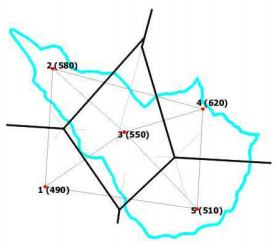
\includegraphics[width=0.7\linewidth]{thiessen1}
		\caption{Triangulacja i~symetralne boków.}
	\end{subfigure}%
	\begin{subfigure}{.5\textwidth}
		\centering
		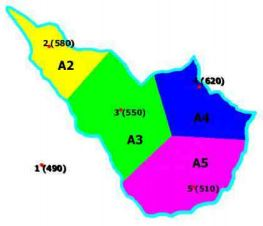
\includegraphics[width=0.7\linewidth]{thiessen2}
		\caption{Wieloboki wyznaczone na obszarze zlewni.}
	\end{subfigure}	
\caption{Schemat dla metody Thiesse. }
\end{figure}

\subsection{Metoda izohiet}
Metoda ta jest polecana dla analizy obszarów górskich, albowiem uwzględnia zależność między wysokością nad poziomem morza, a~wysokością opadu. Uznawana jest również za najbardziej dokładną.

Polega na podziale obszaru zlewni na fragmenty ograniczane przez kolejne izohiety. Dla każdego z~nich przyjmuje się wartość opadu będącą średnią arytmetyczną opadu na wyznaczających dany fragment izohietach. Taką samą zasadę stosuje się gdy granica zlewni przebiega blisko kolejnej izohiety. Jeżeli odległość ta jest znaczna, przyjmuje się wysokość opadu bliższej izohiety. Suma iloczynów wartości opadu i~powierzchni poszczególnych fragmentów stanowi wartość opadu na zadanej powierzchni.


\subsection{Metoda krzywej hipsometrycznej}
Podobnie jak metoda izohiet, zalecana jest dla badania terenów górskich, a~przede wszystkim małych zlewni. Jest stosunkowo pracochłonna, aczkolwiek dokładna.

W IV ćwiartce układu współrzędnych kreślona jest krzywa hipsometryczna oparta na mapie wysokościowej zlewni. Obrazuje ona zależność wysokości nad poziom morza (oś $X$) i~powierzchni zlewni (oś $Y$). Linia w~ćwiartce II nazywana jest krzywą gradientową opadów atmosferycznych. Jest to korelacja wzniesienia posterunku opadowego na osi odciętych oraz wysokości zmierzonego opadu na osi rzędnych.

Dokonując rzutowania krzywej hipsometrycznej poprzez ćwiartkę III i II (w~oparciu o~krzywą gradientową) na ćwiartkę I wyznaczana jest kolejna krzywa (zwana pluwiometryczną). Pole obszaru znajdującego się pod nią to rozmiar opadu na analizowanym obszarze. Opisany proces obrazuje rysunek~\ref{fig:hipsometryczna}.

\begin{figure}[!ht]
\centering
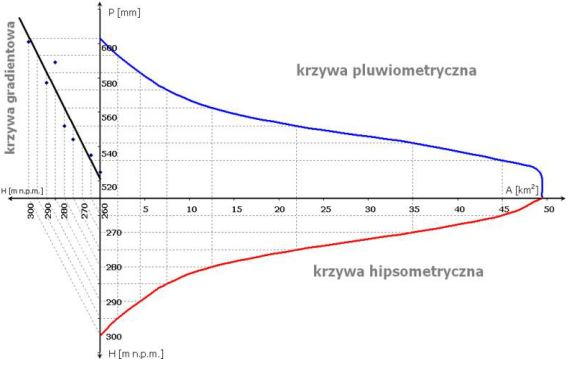
\includegraphics[width=0.7\linewidth]{hipsometryczna}
\caption{Wykres metody hipsometrycznej.}
\label{fig:hipsometryczna}
\end{figure}

\subsection{Metoda regionów opadowych}
Analizując zlewnię pod kątem cech fizyczno-geograficznych wydziela się obszary o~podobnych warunkach pogodowych. Wskazanie opadu na każdym z~nich stanowi średnia arytmetyczna pomiarów z~posterunków opadowych znajdujących się wewnątrz niego. Uwzględniając ograniczenie granicami zlewni wylicza się powierzchnię poszczególnych fragmentów i~mnoży ją przez wskazanie opadu. Podobnie jak w~innych metodach - suma takich iloczynów stanowi wielkość opadu w~zlewni.

Metoda ta jest mniej dokładna. Naturalnie, spisuje się najlepiej gdy obszar zlewni jak najbardziej pokrywa się z~wyznaczonymi regionami. Jej atutem jest niewielki poziom skomplikowania.

\begin{figure}[!ht]
\centering
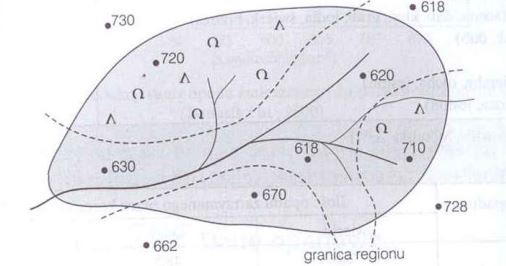
\includegraphics[width=0.5\linewidth]{regiony_opadowe}
\caption{Schemat regionów opadowych (źródło:~\cite{metody_obliczania_pb}).}
\label{fig:regiony_opadowe}
\end{figure}


\section{Zastosowana metoda}
\label{sec:zastosowana_metoda}
Jak wspomniano we wstępie, praca ta traktuje o analizie danych pojedynczego opadu, a~nie zbieranych przez pewien okres czasu. Przy wyborze sposobu przekształcenia danych jest to bardzo istotne kryterium, które wraz z~możliwością jak najlepszego dopasowania do kształtu zlewni stanowiło główne wymagania tej części pracy. Brano także pod uwagę poziom skomplikowania implementacji stosowanego rozwiązania. Wybór padł na połączenie techniki triangulacji wraz z~interpolacją przy użyciu płaszczyzny.

\begin{figure}[!ht]
	\centering
	\includegraphics[scale=0.7]{algorytm}
	\caption{Schemat krokowy zastosowanej metody}
	\label{fig:algorytm}
\end{figure}

%Triangulacja polega na stworzeniu siatki trójkątów o~wierzchołkach w~zadanych punktach (w tym wypadku są to posterunki opadowe o znanej wysokości opadu). 
Zastosowano algorytm triangulacji Delaunay'a, który wprowadza dodatkowe ograniczenie na tworzone trójkąty. Mianowicie, okrąg opisany na każdym z~nich nie może zawierać innych punktów siatki poza wierzchołkami danego trójkąta. Ta metoda ma na celu maksymalizację równoboczności powstałych trójkątów, a~co za tym idzie, równomierność budowanej siatki.

\begin{figure}[!ht]
	\centering
	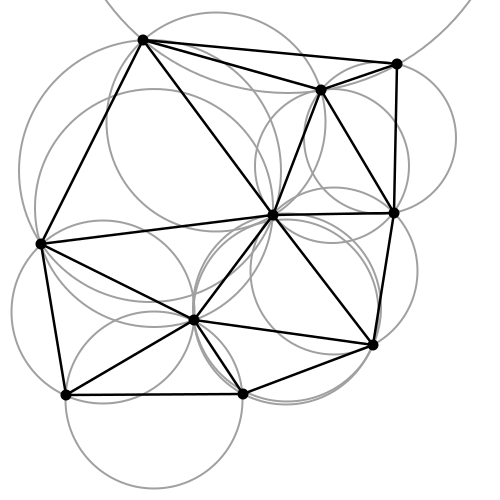
\includegraphics[scale=0.3]{delaunay}
	\caption{Schemat realizacji warunku Delaunay'a (źródło: \textit{www.wikipedia.pl}).}
	\label{fig:delaunay}
\end{figure}

Po zastosowaniu triangulacji, następnym etapem jest wyznaczenie punktów, dla których należy interpolować wartość opadu. Tymi punktami są poszczególne węzły granicy wskazanej zlewni oraz miejsca przecięcia tej granicy z~krawędziami trójkątów. Wraz z~posterunkami opadowymi znajdującymi się wewnątrz obszaru dla jakiego wyznaczany jest opad powierzchniowy będą stanowiły węzły kolejnej triangulacji.

Wyznaczenie wartości dla wskazanych punktów odbywa się poprzez interpolację płaszczyzną przechodzącą przez trzy punkty (będące wierzchołkami kolejnych trójkątów). Ustalane są współrzędne wektorów normalnych dla poszczególnych płaszczyzn (czyli wektorów prostopadłych do powierzchni danej płaszczyzny), a~następnie korzystając ze wzoru~\ref{eq:wartosc_interpolowana}, wyznaczana jest wartość opadu ($z$) w~punkcie o~zadanych współrzędnych~$x$~i~$y$.

Równanie płaszczyzny przedstawia się następująco.

\begin{equation}
\begin{gathered}
A(x - x_0) + B(y - y_0) + C(z - z_0) = 0 \\
[A, B, C] = (P_2 - P_1) \times (P_3 - P_2)
\label{eq:rownanie_plaszczyzny}
\end{gathered}
\end{equation}
gdzie
% eqwhere z aghdpl powoduje błąd
\begin{description}[leftmargin=3cm, itemsep=0cm, labelsep=0cm]
	\item[$x_0, y_0, z_0$] współrzędne punktu należącego do płaszczyzny,
	\item[{[}$A, B, C${]}] wektor normalny płaszczyzny, %rozwiązać problem z [ ] jako wektor
	\item[$A, B, C$] nie mogą być jednocześnie równe 0.
\end{description}
%
Co po przekształceniu daje
\begin{equation}
\label{eq:wartosc_interpolowana}
	z = \frac{A(x - x_0) + B(y - y_0)}{-C} + z_0
\end{equation}
gdzie $C \neq 0$.


Jeżeli $C$, ze wzoru~\ref{eq:wartosc_interpolowana}, przyjmuje wartość 0 oznacza to, iż w~każdym wierzchołku trójkąta opad był zerowy. Wówczas punktowi interpolowanemu przypisuje się takowe wskazanie.

Po przeprowadzeniu interpolacji wartości dokonuje się ponownej triangulacja, tym razem z~użyciem punktów interpolowanych oraz posterunków wewnątrz zlewni. Nowopowstała siatka trójkątów, wraz z~trzecim wymiarem jakim jest wysokość opadu, tworzy zbiór brył o~trójkątnych podstawach. Wyznaczając i~sumując objętość opadu w~każdej z~nich uzyskiwany jest łączny opad na wskazanej zlewni~\cite{matematyka_poradnik, mathMonthly}.

\begin{equation}
	V = \sum_{i=1}^{n}P_{pi}*\frac{h_{i1}+h_{i2}+h_{i3}}{3}
\label{eq:opad_powierzchniowy}
\end{equation}
gdzie
\begin{description}[leftmargin=3cm, itemsep=0cm, labelsep=0cm]
	\item[$V$] łączna objętość opadu,
	\item[$n$] ilość wyznaczonych brył,
	\item[$P_{pi}$] pole podstawy $i$-tej bryły,
	\item[$h_{i1}, h_{i2}, h_{i3}$] długość krawędzi bocznej $i$-tej bryły (wartość opadu) w~danym wierzchołku.
\end{description}




\section{Możliwe rozszerzenia algorytmu}
Oczywiście można dążyć do usprawnienia metody przekształcania danych wejściowych.
Przykładowe rozszerzenia mogą obejmować
\begin{itemize}
\item{ Analizę sąsiednich dla trójkąta punktów i~na ich podstawie wyznaczenie wartości opadu w~środku zadanego fragmentu, a~dalej dzielenie go na mniejsze. }

\item{ Interpolację powierzchnią inną niż płaszczyzna. Kształt powierzchni definiować na bazie większej ilości punktów znanych. }

\item{ Uwzględnienie ukształtowania terenu podczas analizy obszaru zlewni. }
\end{itemize}
\chapter{Implementacja}
Jak wspomniano w poprzednim rozdziale, dane wejściowe są wskazaniami pomiarów z~poszczególnych posterunków opadowych. Są to dane punktowe, zatem aby oszacować ilość wody jaka spadła na zadanym obszarze konieczne jest przeprowadzenie ich interpolacji w~celu aproksymacji wartości dla punktów stanowiących granicę wskazanej zlewni, co dalej zmierza do wyznaczenia opadu powierzchniowego.

Istnieje wiele metod wyznaczania średniego opadu powierzchniowego. Począwszy od prostego obliczenia średniej arytmetycznej wartości z~posterunków opadowych, poprzez metody wieloboków Voronoia, izohiet po hipsometryczną. Różnią się one dokładnością, sposobem aproksymacji czy też zaawansowaniem danych wejściowych.

Jak wspomniano we wstępie, praca ta traktuje o analizie danych pojedynczego opadu, a~nie zbieranych przez pewien okres czasu. Przy wyborze sposobu przekształcenia danych jest to bardzo istotne kryterium, które wraz z~możliwością jak najlepszego dopasowania do kształtu zlewni stanowiło główne wymagania tej części pracy.

%\section{Triangulacja i algorytm Delaunay'a}
%Do przeprowadzenia interpolacji danych punktowych zastosowano technikę triangulacji. Polega ona na stworzeniu siatki trójkątów o~wierzchołkach w punktach z~wartością znaną (wysokość opadu na posterunku opadowym). Wybór padł na zastosowanie algorytmu Delaunay'a, który wprowadza dodatkowe ograniczenie na tworzone trójkąty. Mianowicie, okrąg opisany na każdym z~nich nie może zawierać innych punktów siatki poza wierzchołkami danego trójkąta. Ta metoda ma na celu maksymalizację równoboczności powstałych trójkątów, a~co za tym idzie, równomierność budowanej siatki.

\section{Zastosowana metoda}
Wybór padł na połączenie techniki triangulacji wraz z~interpolacją przy użyciu płaszczyzny.

Triangulacja polega na stworzeniu siatki trójkątów o~wierzchołkach w~zadanych punktach (w tym wypadku są to posterunki opadowe o znanej wysokości opadu). Zastosowano algorytm Delaunay'a, który wprowadza dodatkowe ograniczenie na tworzone trójkąty. Mianowicie, okrąg opisany na każdym z~nich nie może zawierać innych punktów siatki poza wierzchołkami danego trójkąta. Ta metoda ma na celu maksymalizację równoboczności powstałych trójkątów, a~co za tym idzie, równomierność budowanej siatki.

\begin{figure}[ht]
	\centering
	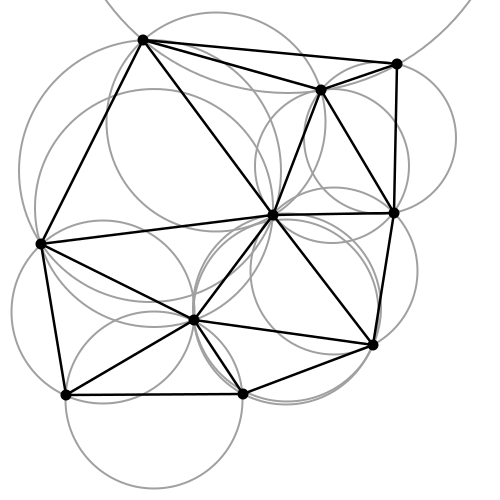
\includegraphics[scale=0.3]{delaunay}
	\caption{Schemat zastosowania algorytmu Delaunay'a (źródło: wikipedia)}
	\label{fig:delaunay}
\end{figure}

\begin{figure}[ht]
	\centering
\begin{subfigure}[t]{.5\textwidth}
	\centering
	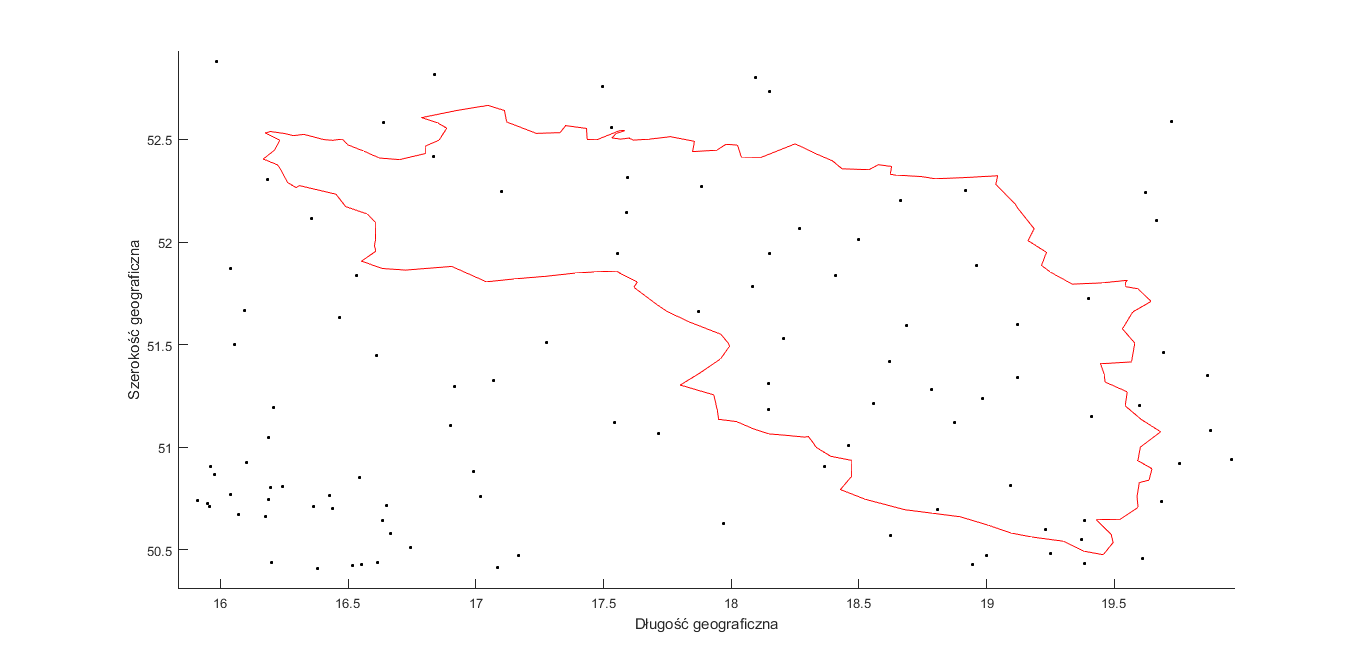
\includegraphics[width=0.7\linewidth]{dane_wejsciowe}
	\caption{Posterunki opadowe i~obszar zlewni}
	\label{fig:dane_wejsciowe}
\end{subfigure}	
	\begin{subfigure}[t]{0.5\textwidth}
	\centering
	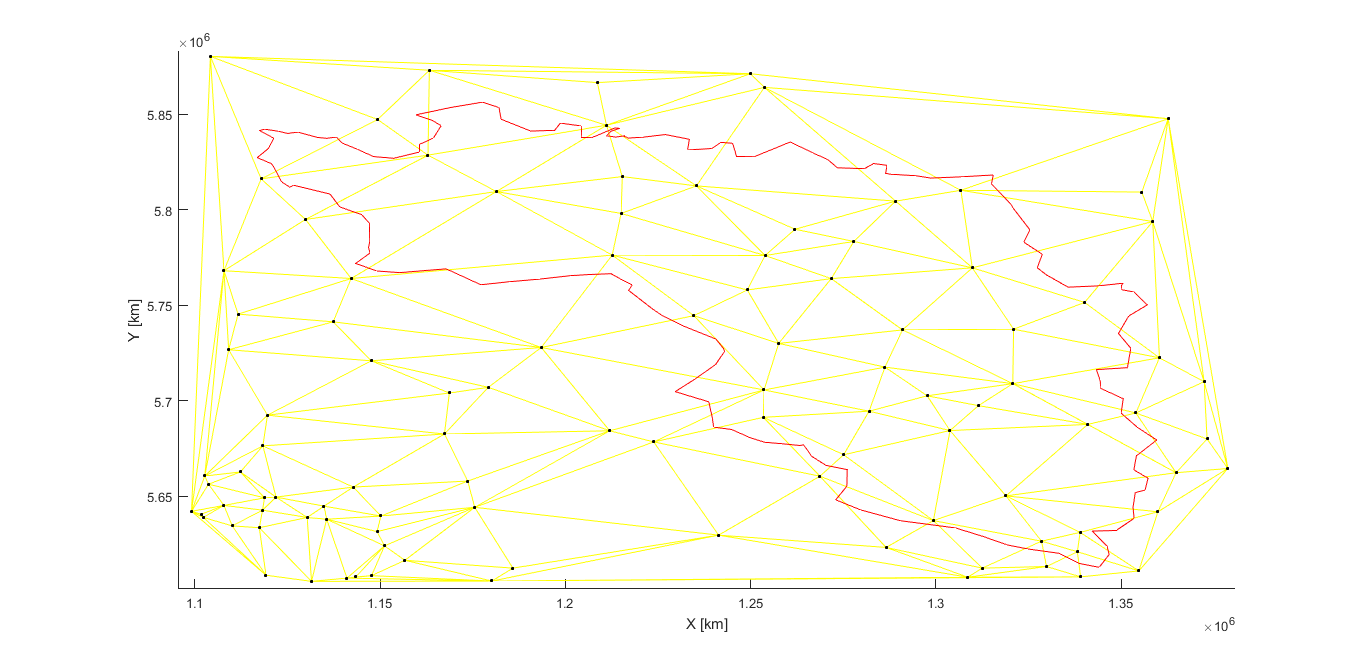
\includegraphics[width=0.7\linewidth]{triangulacja_zlewnia}
	\caption{Siatka triangulacji dla posterunków}
	\label{fig:triagnulacja_danych}
\end{subfigure}	
\caption{Prezentacja danych wejściowych}
	
\end{figure}

Po zastosowaniu triangulacji następnym etapem jest wyznaczenie punktów, dla których należy interpolować wartość opadu. Tymi punktami są poszczególne węzły granicy wskazanej zlewni oraz miejsca przecięcia tej granicy z krawędziami trójkątów. Wraz z~posterunkami opadowymi znajdującymi się wewnątrz obszaru dla jakiego wyznaczany jest obszar powierzchniowy będą stanowiły węzły kolejnej triangulacji.


\begin{figure}[ht]
	\centering
	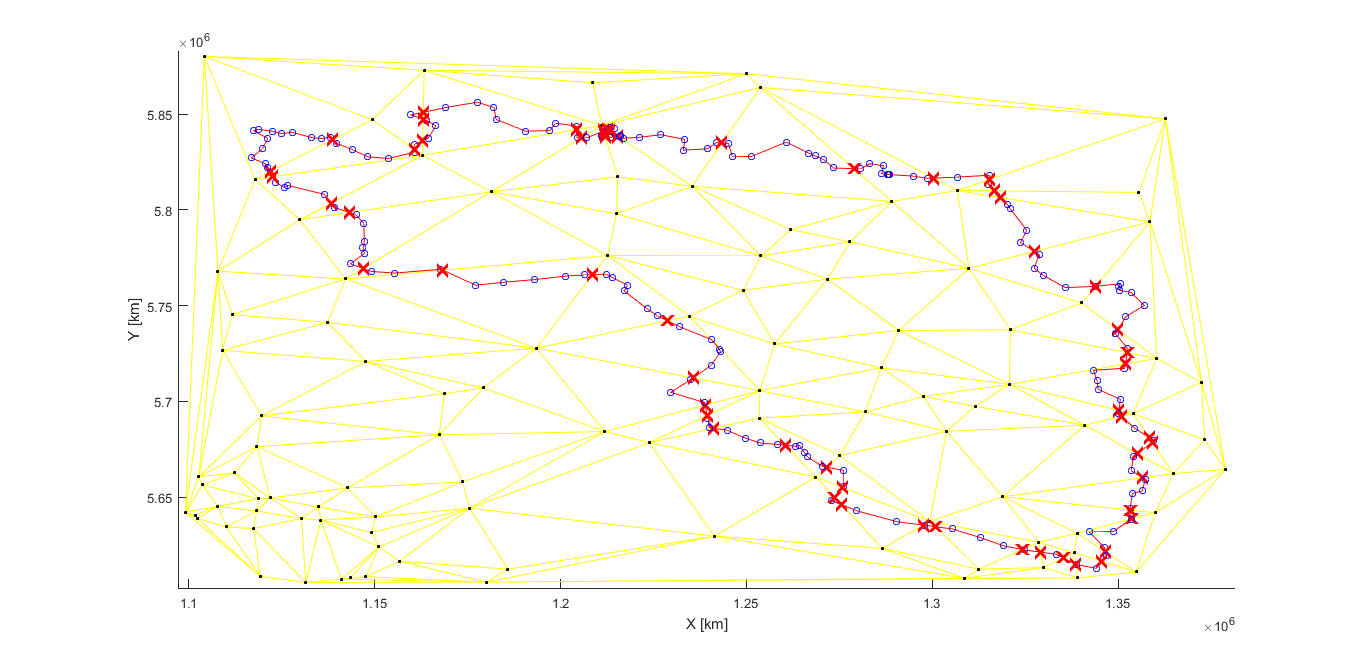
\includegraphics[scale=0.5]{punkty_do_interpolacji}
	\caption{Punkty wyznaczone do interpolacji.
	O - węzły granicy, X - przecięcia granicy z~liniami siatki.}
	\label{fig:punkty_interpolacji}
\end{figure}

Jak wspomniano na początku tego rozdziału, wyznaczenie wartości dla powstałych punktów odbywa się poprzez interpolację powierzchniową poszczególnych trójkątów.

Została stworzona funkcja wyznaczająca wektor normalny dla pojedynczego trójkąta. Wektor normalny jest prostopadły do powierzchni zadanej płaszczyzny. Z~jego pomocą (oraz znając współrzędne punktu należącego do płaszczyzny - np. jeden z~wierzchołków trójkąta) wyznacza się wartość \textit{z} punktu o~współrzędnych $x$~i~$y$~w~oparciu o~równanie ogólne płaszczyzny.

\begin{equation*}
\begin{gathered}
A(x - x_0) + B(y - y_0) + C(z - z_0) = 0 \\
[A, B, C] = (P_2 - P_1) \times (P_3 - P_2)
\label{eq:rownanie_plaszczyzny}
\end{gathered}
\end{equation*}
gdzie
% eqwhere z aghdpl powoduje błąd
\begin{description}[leftmargin=3cm, itemsep=0cm, labelsep=0cm]
	\item[$x_0, y_0, z_0$] współrzędne punktu należącego do płaszczyzny
	\item[$A, B, C$] współrzędne wektora normalnego
\end{description}

Przy użyciu przygotowanej funkcji, dla wszystkich wyznaczonych do interpolacji punktów uzyskiwana jest wartość opadu korzystając ze współrzędnych $x$~i~$y$ punktu i~wektora normalnego trójkąta, w~którym ten punkt się znajduje.

\begin{figure}[ht]
	\centering
	\includegraphics[scale=0.5]{algorytm}
	\caption{Schemat krokowy zastosowanej metody}
	\label{fig:algorytm}
\end{figure}

\begin{figure}[ht]
	\centering
	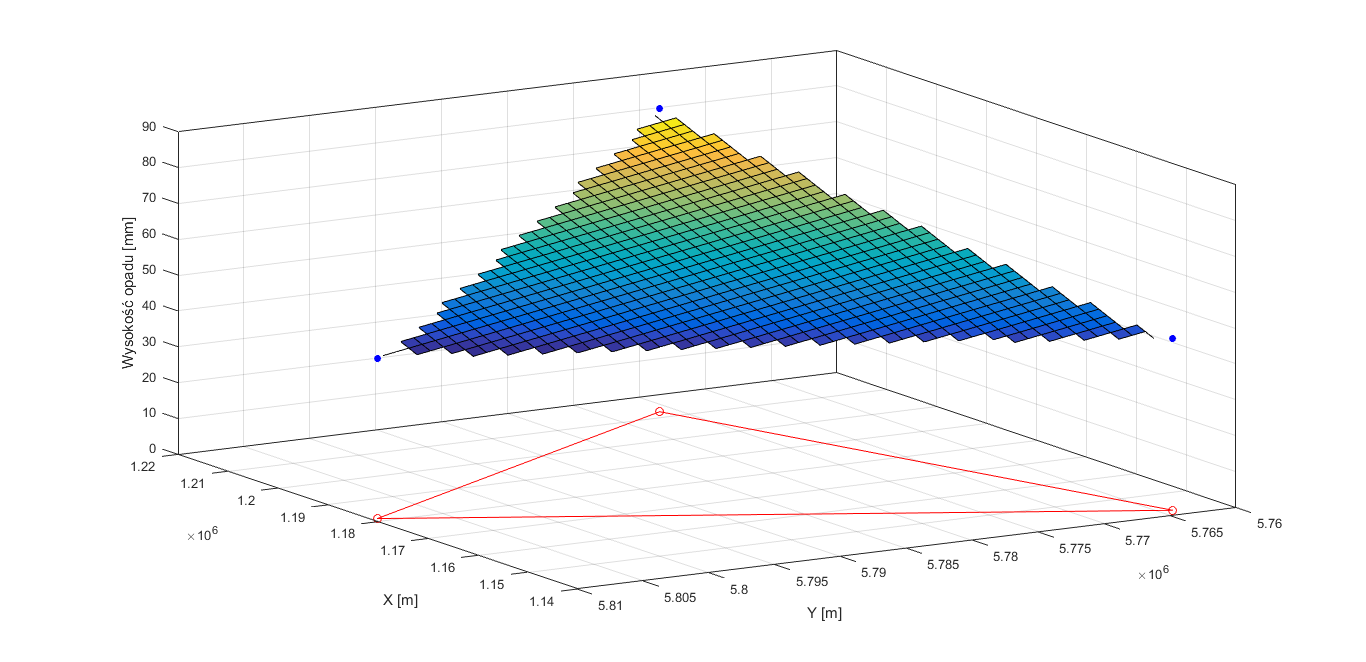
\includegraphics[scale=0.5]{prezentacja_interpolacji}
	\caption{Interpolacja płaszczyzną dla pojedynczego trójkąta}
	\label{fig:plaszczyzna_interpolacji}
\end{figure}

Po zakończeniu interpolacji wartości przeprowadzana jest ponowna triangulacja mająca na celu stworzenie brył o~trójkątnej podstawie (wysokości brył to wartość opadu w~punkcie będącym wierzchołkiem). Tym razem zastosowane zostaną punkty interpolowane oraz posterunki wewnątrz zlewni. Jak zaprezentowano na rysunku~\ref{fig:druga_triangulacja}, pojawia się komplikacja


\begin{figure}[ht]
	\centering
	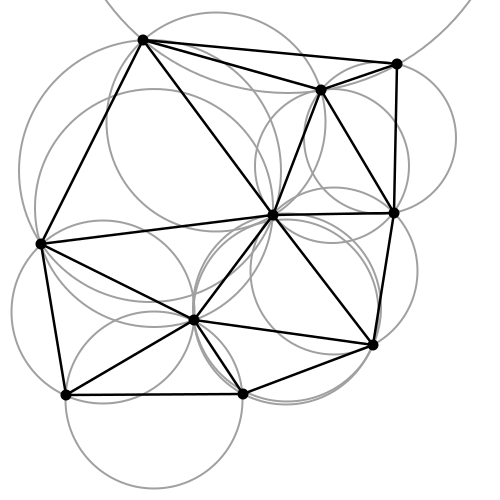
\includegraphics[scale=0.3]{delaunay}
	\caption{Schemat zastosowania algorytmu Delaunay'a (źródło: wikipedia)}
	\label{fig:delaunay}
\end{figure}

\begin{figure}[ht]
	\centering
\begin{subfigure}[t]{.5\textwidth}
	\centering
	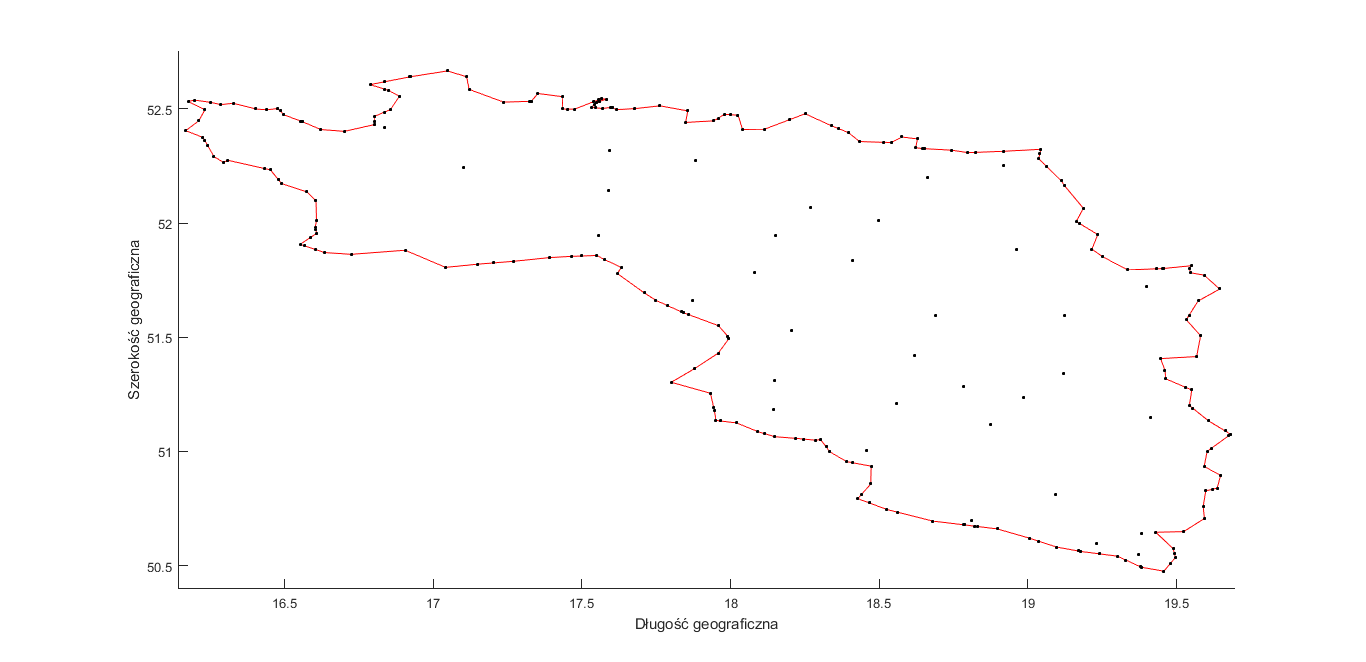
\includegraphics[width=0.7\linewidth]{dane_druga_triangulacja}
	\caption{Punkty dla ponownej triangulacji}
	\label{fig:dane_wejsciowe}
\end{subfigure}	
	\begin{subfigure}[t]{0.5\textwidth}
	\centering
	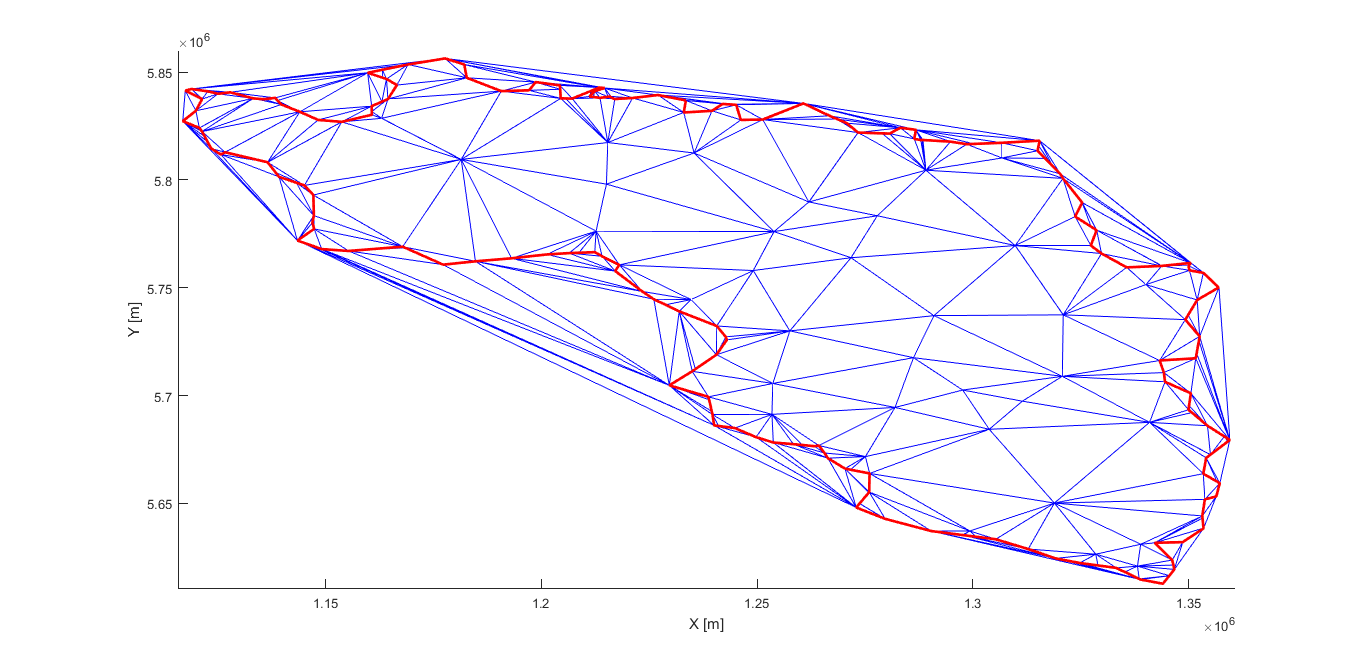
\includegraphics[width=0.7\linewidth]{druga_triangulacja}
	\caption{Siatka triangulacji dla wyznaczonych punktów}
	\label{fig:druga_triagnulacja}
\end{subfigure}	
\caption{Triangulacja danych interpolowanych}
	
\end{figure}
\chapter{Opracowanie wyników}

Rozdział ten zawiera analizę wyników opisanego w~części~\ref{cha:implementacja}.


\section{Wielkość błędu}
asdasd

\section{Warianty opadu}

\section{Analiza wrażliwości na posterunki opadowe}
W~tej części przeprowadzono wpływ wyłączenia wskazanego posterunku opadowego (ograniczono się do wybory punktów zawartych w granicach wskazanej zlewni) na wynik działania omawianej metody. Pozwala to znaleźć odpowiedź na pytanie: \textit{Czy sieć istniejących posterunków opadowych jest wystarczająca?}, a~to pomoże podejmować decyzje o~zwiększaniu ilości owych posterunków bądź przeniesieniu w~inną lokalizację.

Rysunek~\ref{fig:identyfikatory} przedstawia identyfikatory wykluczanych z~analizy punktów, natomiast wiersze tabeli prezentują rezultat działania programu bez zadanego punktu.

\begin{figure}[ht]
	\centering
	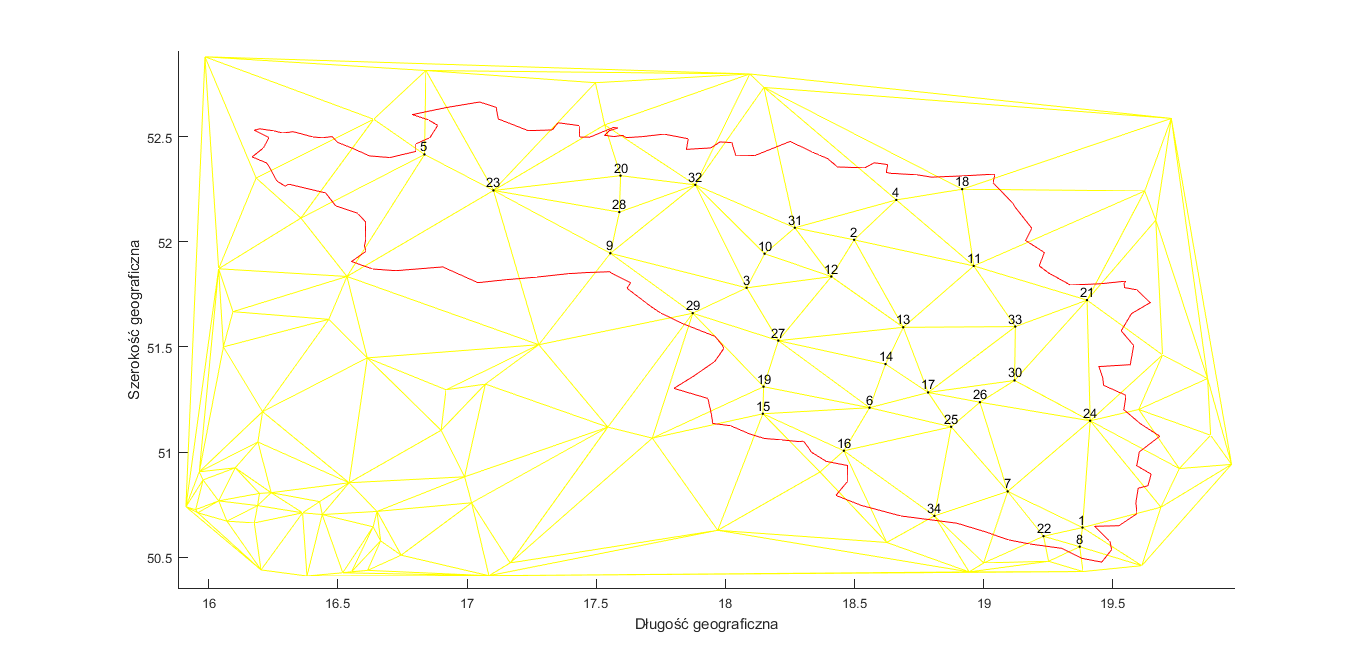
\includegraphics[width=1\linewidth]{identyfikatory_punktow}
	\label{fig:identyfikatory}
	\caption{Identyfikatory posterunków wewnątrz zlewni}
\end{figure}

\subsection{Wniosek}
\chapter{Podsumowanie}
\chapter{Słownik pojęć}
\begin{description}[leftmargin=5cm]
\item[Posterunek opadowy] \hfill \\ 
Miejsce przeprowadzania pomiarów i obserwacji meteorologicznych. Mierzona jest ilość wody opadowej, która zebrała się w~deszczomierzu.
\item[Posterunek wodowskazowy] \hfill \\ 
Miejsce prowadzenia pomiarów stanu wody za pomocą wodowskazu.
\item[Profil wodowskazowy] \hfill \\ 
Punkt na rzece, w~którym zamontowany jest wodowskaz.
\item[Zlewnia] \hfill \\ 
Obszar, z którego wody spływają do jednego punktu danego zbiornika wodnego lub jego fragmentu.
\item[Zbiornik retencyjny] \hfill \\
Sztuczny zbiornik wodny powstały w wyniku zatamowania wód rzecznych przez zaporę. Pełnić może wiele funkcji, takich jak przeciwpowodziowa energetyczna czy nawet rekreacyjna.
\end{description}
\chapter{Dodatek A - fragmenty kodów źródłowych}
\label{cha:dodatek_A}
\section{Odczyt danych z serwisu}
\label{sec:kod_odczyt_danych}
\section{Interpolacja}
\section{inny podrozdzial}

%\include{tests}
\bibliographystyle{abbrv}
\bibliography{bibliografia}

\end{document}
